\documentclass[a4paper]{article}
\usepackage[spanish]{babel}
\usepackage[pdftex,usenames,dvipsnames]{color}
\usepackage{multicol}
\usepackage{graphicx}
\usepackage{listings}
\usepackage{color}
\usepackage{hyperref}

\definecolor{dkgreen}{rgb}{0,0.6,0}
\definecolor{gray}{rgb}{0.5,0.5,0.5}
\definecolor{mauve}{rgb}{0.58,0,0.82}

\lstset{
    language=bash, 
    basicstyle=\footnotesize\color{black},
    backgroundcolor=\color{white},
    morekeywords={durar@durar, restart}, keywordstyle=\color{green},
    classoffset=1,
    showspaces=false,
    showstringspaces=false,
    showtabs=false,
    frame=single, 
    tabsize=2,
    captionpos=b,
    breaklines=true,
}
\lstdefinestyle{bashCentOS}{
    language=bash, 
    basicstyle=\footnotesize\color{black},
    backgroundcolor=\color{white},
    morekeywords={durar@localhost, start}, keywordstyle=\color{red},
    classoffset=1,
    showspaces=false,
    showstringspaces=false,
    showtabs=false,
    frame=single, 
    tabsize=2,
    captionpos=b,
    breaklines=true,
}

\begin{document}
\pagestyle{plain}
\title{Práctica 4: Benchmarking y Ajuste del Sistema" \\ 
Ingeniería de Servidores}
\author{Raúl Durán Racero}
\begin{figure}
    \raggedright
    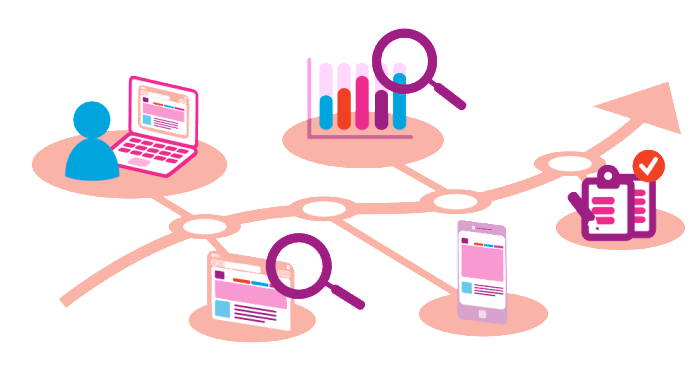
\includegraphics[width=1.25\textwidth]{benchmarking004.png}
\end{figure}
\maketitle
\begin{figure}
    \centering
    \includegraphics[width=0.25\textwidth]{logoEtsiit.pdf}
\end{figure}

\newpage
\tableofcontents
\newpage
\section{Ejercicio 1}
Una vez que haya indagado sobre los benchmarks disponibles, seleccione 
como mínimo dos de ellos y proceda a ejecutarlos en Ubuntu y CentOS.
Comente las diferencias.
\subsection{Phoronix en UbuntuServer}
Lo primero que haremos será obtener el paquete de la página de Phoronix e instalarlo:
\begin{lstlisting}
    durar@durar:~$ sudo wget http://phoronix-test-suite.com/releases/repo/pts.debian/files/phoronix-test-suite_10.6.1_all.deb
    durar@durar:~$ sudo dpkg -i phoronix-test-suite_10.6.1_all.deb
\end{lstlisting}
Una vez instalado, podemos ver los diferentes tests y suites que dispone Phoronix:
\begin{lstlisting}
    durar@durar:~$ phoronix-test-suite list-available-tests
    durar@durar:~$ phoronix-test-suite list-available-suites
\end{lstlisting}
De la lista de tests, escogeremos dos. En mi caso, he escogido los siguientes:
\subsection*{\textbf{pts/sudokut:}}
Sudokut es un test que mide cuánto tiempo tarda el sistema en resolver 100 puzzles 
\textsl{Sudoku} escritos en TCL (\textsl{Tool Command Language}):
\begin{lstlisting}
    durar@durar:~$ phoronix-test-suite benchmark pts/sudokut 
\end{lstlisting}
\subsection*{\textbf{pts/ramspeed:}}
RAMspeed SMP comprueba como actúa la RAM de nuestro sistema:
\begin{lstlisting}
    durar@durar:~$ phoronix-test-suite benchmark pts/ramspeed 
\end{lstlisting}
Nos pedirá que escojamos distintas ocpiones. Escogemos las que queramos (en mi caso, 
solo compararé la función \textsl{Add}):

Si hay errores a la hora de instalar las dependencias necesarias para los tests, 
intenta actualizar:
\begin{lstlisting}
    durar@durar:~$ sudo apt-get update
\end{lstlisting}

\subsection{Phoronix en CentOS}
Repetimos los pasos de instalación que hicimos en UbuntuServer (si tienes instalados
en CentOS wget y dpkg):
\begin{lstlisting}[style=bashCentOS]
    [durar@localhost ~]$ sudo wget http://phoronix-test-suite.com/releases/repo/pts.debian/files/phoronix-test-suite_10.6.1_all.deb
    [durar@localhost ~]$ sudo dpkg -i phoronix-test-suite_10.6.1_all.deb
\end{lstlisting}
Y volvemos a comrpobar los tests y suites:
\begin{lstlisting}[style=bashCentOS]
    [durar@localhost ~]$ phoronix-test-suite list-available-tests
    [durar@localhost ~]$ phoronix-test-suite list-available-suites
\end{lstlisting}
Ejecutaremos los mismos tests que en UbuntuServer para comparar resultados:
\begin{lstlisting}[style=bashCentOS]
    [durar@localhost ~]$ phoronix-test-suite benchmark pts/sudokut
    [durar@localhost ~]$ phoronix-test-suite benchmark pts/ramspeed
\end{lstlisting}

\subsection{Comparación de Resultados}
\subsection*{\textbf{Sudokut:}}
\begin{figure}[hbt!]
    \centering
    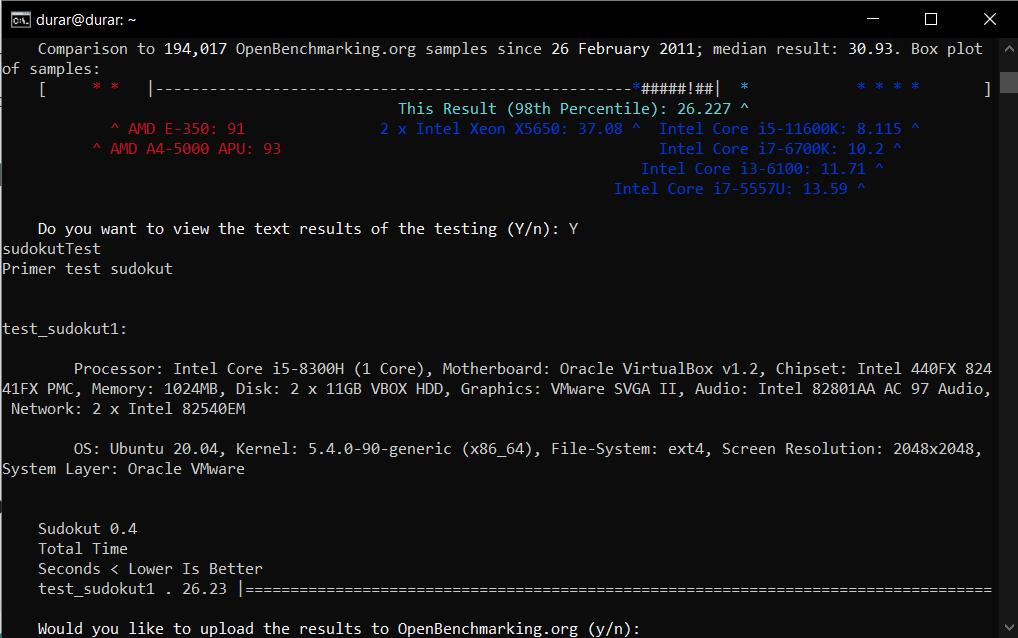
\includegraphics[width=\textwidth]{resultado_sudokut1.png}
    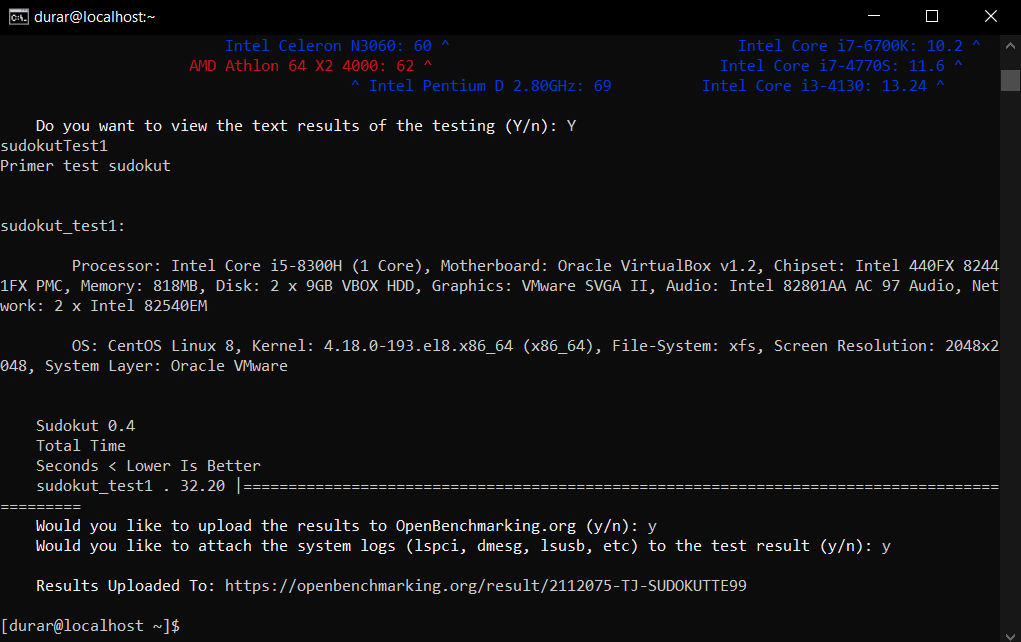
\includegraphics[width=\textwidth]{resultado_sudokut_centos.png}
\end{figure}
Podemos ver como en la primera imagen (UbuntuServer), el test Sudokut ha tardado menos 
en ejecutarse (26.23s) que en CentOS (32.29s).
\subsection*{\textbf{RAMspeed:}}
\begin{figure}[hbt!]
    \centering
    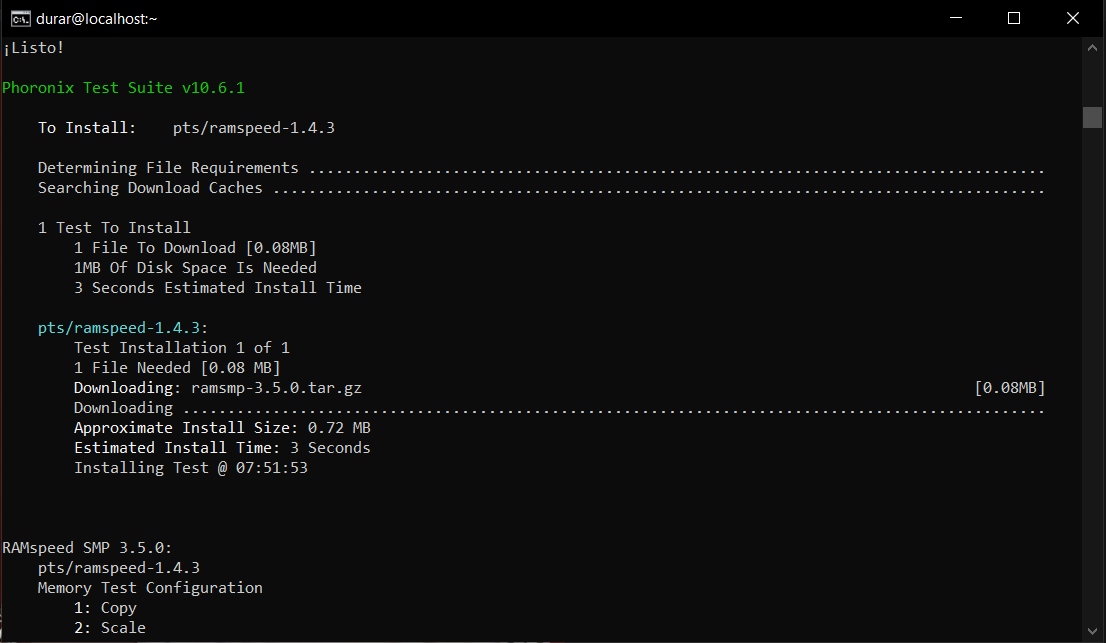
\includegraphics[width=\textwidth]{ramspeed Centos1.png}
\end{figure}
\newpage
\section{Ejercicio 2}
Tras probar un test básico para una web, utilizaremos Jmeter para hacer 
un test sobre una aplicación que ejecuta sobre dos contenedores (uno
para la BD y otro para la aplicación en sí). El código está disponible en 
\href{https://github.com/davidPalomar-ugr/iseP4JMeter}{https://github.com/davidPalomar-ugr/iseP4JMeter}
donde se dan detalles sobre cómo ejecutar la aplicación en una de nuestras máquinas virtuales.


\section{Ejercicio Opcional}
Con esta información usted podría modificar los parámetros
de configuración de Apache, PHP o MariaDB para observar un cambio en el
comportamiento del servidor (CentOS o Ubuntu server) mediante la aplicación
de un benchmark y analizando el cambio en las prestaciones o mediante el análisis
de datos de monitorización ante una carga aplicada.

\newpage
\begin{thebibliography}{99}
    \bibitem[Descargar Phoronix]{descargar phoronix} 
    \href{https://www.phoronix-test-suite.com/}{https://www.phoronix-test-suite.com/}
    \bibitem[Instalar Phoronix Ubuntu]{pagina ubuntuwiki para instalar phoronix}
    \href{https://wiki.ubuntu.com/PhoronixTestSuite#installing}{https://wiki.ubuntu.com/PhoronixTestSuite\#installing}
    \bibitem[OpenBenchmarking]{openbenchmarking} 
    \href{https://openbenchmarking.org/s}{https://openbenchmarking.org/s}
    \bibitem[Codigo JMeter]{codigo github para Jmeter} 
    \href{https://github.com/davidPalomar-ugr/iseP4JMeter}{https://github.com/davidPalomar-ugr/iseP4JMeter}
    \bibitem[Apache JMeter]{pag oficial de jmeter} 
    \href{https://jmeter.apache.org/}{https://jmeter.apache.org/}
    \bibitem[]{} 
    \href{}{}
\end{thebibliography}
\end{document}